\subsection{Multidimensional likelihood estimator (PDE range-search approach)}
\label{sec:pders}

This is a generalization of the projective likelihood classifier described in
Sec.~\ref{sec:likelihood} to $\Nvar$ dimensions, where $\Nvar$ is
the number of input variables used. If the multidimensional 
PDF\index{PDE-RS, multidimensional likelihood} 
for signal and background (or regression data) were known, this classifier 
would exploit the full information contained in the input variables, and  
would hence be optimal. In practice however, huge training samples are necessary 
to sufficiently populate the multidimensional phase space.\footnote
{
	Due to correlations between the input variables, only a sub-space of 
	the full phase space may be populated.
} 
Kernel estimation methods may be used to approximate the shape of the PDF
for finite training statistics.

A simple probability density estimator\index{PDE} denoted {\em PDE range search}, or {\em PDE-RS}, 
has been suggested in Ref.~\cite{CarliKoblitz}. The PDE for a given test event (discriminant) 
is obtained by counting the (normalised) number of 
training events that occur in the "vicinity" of the test event. The 
classification of the test event may then be conducted on the basis of the 
majority of the nearest training events. The $\Nvar$-dimensional
volume that encloses the "vicinity" is user-defined and can be adaptive. A search method 
based on sorted binary trees is used to reduce the computing time for the 
range search. To enhance the sensitivity within the volume, kernel 
functions are used to weight the reference events according to their 
distance from the test event. PDE-RS is a variant of the k-nearest neighbour
classifier described in Sec.~\ref{sec:knn}.

\subsubsection{Booking options}

The PDE-RS classifier is booked via the command:
\begin{codeexample}
\begin{tmvacode}
factory->BookMethod( Types::kPDERS, "PDERS", "<options>" );
\end{tmvacode}
\caption[.]{\codeexampleCaptionSize Booking of PDE-RS: the first argument is a predefined 
		   enumerator, the second argument is a user-defined 
		   string identifier, and the third argument is the configuration options string.
         Individual options are separated by a ':'. 
         See Sec.~\ref{sec:usingtmva:booking} for more information on the booking.}
\end{codeexample}

The configuration options for the PDE-RS classifier are given in 
Option Table~\ref{opt:mva::pders}.

% ======= input option table ==========================================
\begin{option}[t]
\input optiontables/MVA__PDERS.tex
\caption[.]{\optionCaptionSize 
     Configuration options reference for MVA method: {\em PDE-RS}.
     Values given are defaults. If predefined categories exist, the default category 
     is marked by a '$\star$'. The options in Option Table~\ref{opt:mva::methodbase} on 
     page~\pageref{opt:mva::methodbase} can also be configured.     
}
\label{opt:mva::pders}
\end{option}
% =====================================================================
\subsubsection{Description and implementation}

\subsubsection*{Classification}

To classify an event as being either of signal or of background type, a {\em local}
estimate of the probability density of it belonging to either class is 
computed. The method of PDE-RS provides such an estimate by defining a 
volume ($V$) around the test event ($i$), and by counting the number of signal 
($n_S(i,V)$) and background events ($n_B(i,V)$) obtained from the training 
sample in that volume. The ratio 
\beq
\label{eq:PDERSratio}
	\RPDERS(i,V) = \frac{1}{1 + r(i,V)}\,,
\eeq
is taken as the estimate, where $r(i,V)=(n_B(i,V)/N_B)\cdot(N_S/n_S(i,V))$, 
and $N_{S(B)}$ is the total number of signal (background) events in the 
training sample. The estimator $\RPDERS(i,V)$ peaks at 1 (0) for signal 
(background) events. The counting method averages over the PDF within $V$, 
and hence ignores the available shape information inside (and outside) that 
volume.

\subsubsection*{Binary tree search}

Efficiently searching for and counting the events that lie inside the
volume is accomplished with the use of a $\Nvar$-variable binary tree 
search algorithm~\cite{BinaryTree} (\cf\  
Sec.~\ref{sec:binaryTrees}).

\subsubsection*{Choosing a volume}

The TMVA implementation of PDE-RS optionally provides four different 
volume definitions selected via the configuration option \code{VolumeRangeMode}.
\begin{itemize}

\item	\code{Unscaled} \\
		The simplest volume definition consisting of a rigid box of size \code{DeltaFrac},
      in units of the variables.
		This method was the one originally used by the developers of 	
		PDE-RS~\cite{CarliKoblitz}.

\item \code{MinMax} \\ 
		The volume is defined in each dimension (\ie, input variable) 
      with respect to the full range of values found for that dimension
		in the training sample. The fraction of this volume used 
		for the range search is defined by the option \code{DeltaFrac}.

\item \code{RMS} \\
		The volume is defined in each dimension with respect 
		to the RMS of that dimension (input variable), estimated from the 
		training sample. The fraction of this volume used 
		for the range search is defined by the option \code{DeltaFrac}.

\item	\code{Adaptive} \\ 
		A volume is defined in each dimension
		with respect to the RMS of that dimension, estimated from the 
		training sample. The overall scale of the volume is  
		adjusted individually for each test event such 
		that the total number of events confined in the volume lies within 
		a user-defined range (options \code{NEventsMin/Max}). The adjustment
		is performed by the class \code{RootFinder}, which is a C++ implementation
		of Brent's algorithm (translated from the CERNLIB function RZERO).
		The maximum initial volume (fraction of the RMS) and the maximum
		number of iterations for the root finding is set by the options 
		\code{InitialScale} and \code{MaxVIterations}, respectively. The
		requirement to collect a certain number of events in the volume 
		automatically leads to small volume sizes in strongly populated 
		phase space regions, and enlarged volumes in areas where the
		population is scarce.			

\end{itemize}
Although the adaptive volume adjustment is more flexible and should perform
better, it significantly increases the computing time of the PDE-RS discriminant.
If found too slow, one can reduce the number of necessary iterations by 
choosing a larger \code{NEventsMin/Max} interval.

\subsubsection*{Event weighting with kernel functions\index{Kernel estimation}}

One of the shortcomings of the original PDE-RS implementation is its 
sensitivity to the exact location of the sampling volume boundaries: an
infinitesimal change in the boundary placement can include or exclude a 
training event, thus changing $r(i,V)$ by a finite amount.\footnote
{
	Such an introduction of artefacts by having sharp boundaries in the 
	sampled space is an example of Gibbs's phenomenon, and is commonly 
   referred to as {\em ringing} or {\em aliasing}. 
} 
In addition, the shape information within the volume is ignored.

Kernel functions mitigate these problems by weighting each event within
the volume as a function of its distance to the test event. The 
farer it is away, the smaller is its weight. The following kernel functions are
implemented in TMVA, and can be selected with the option \code{KernelEstimator}.
\begin{itemize}

\item	\code{Box} \\
		Corresponds to the original rectangular volume element 
		without application of event weights.

\item \code{Sphere} \\
		A hyper-elliptic volume element is used
		without application of event weights. The hyper-ellipsoid corresponds 
		to a sphere of constant fraction in the \code{MinMax} or \code{RMS}
		metrics. The size of the sphere can be chosen adaptive, just as 
		for the rectangular volume.

\item	\code{Teepee} \\
		The simplest linear interpolation that eliminates the discontinuity 
      problem of the box. The training events are 
      given a weight that decreases linearly with their distance
      from the centre of the volume (the position of the test event).
		In other words: these events are convolved with the triangle 
      or tent function, becoming a sort of teepee in multi-dimensions.

\item \code{Trim} \\ 
      Modified Teepee given by the function $(1-\hat x^3)^3$, where $\hat x$
      is the normalised distance between test event and reference. 

\item \code{Gauss} \\ 
		The simplest well behaved convolution kernel.
		The width of the Gaussian (fraction of the volume size) can be 
		set by the option \code{GaussSigma}.

\end{itemize}
Other kernels implemented for test purposes are ``Sinc'' and 
''Lanczos'' functions $\propto \sin x/x$ of different (symmetric) orders.
They exhibit strong peaks at zero and oscillating tails. The Gaussian and 
Teepee kernel functions are shown in Fig.~\ref{fig:pdersKernels}.

\begin{figure}[t]
\begin{center}
   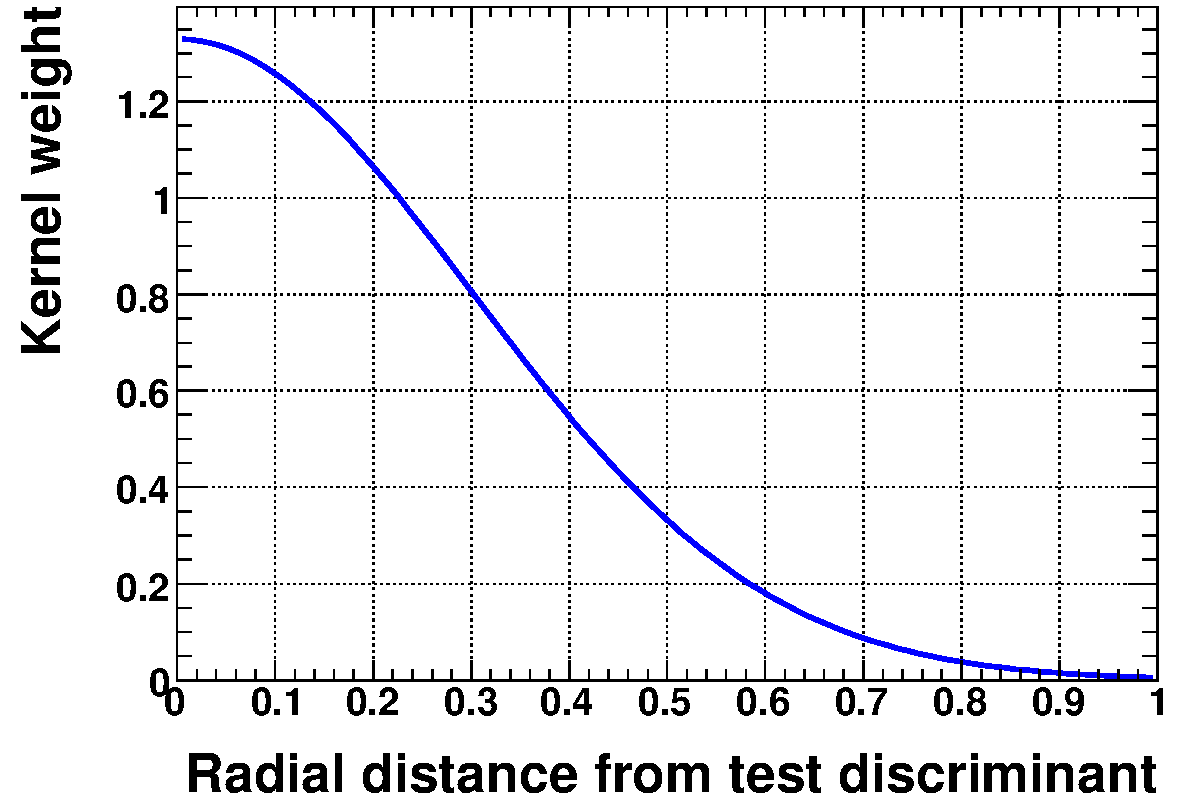
\includegraphics[width=0.49\textwidth]{plots/pders_gauss}
   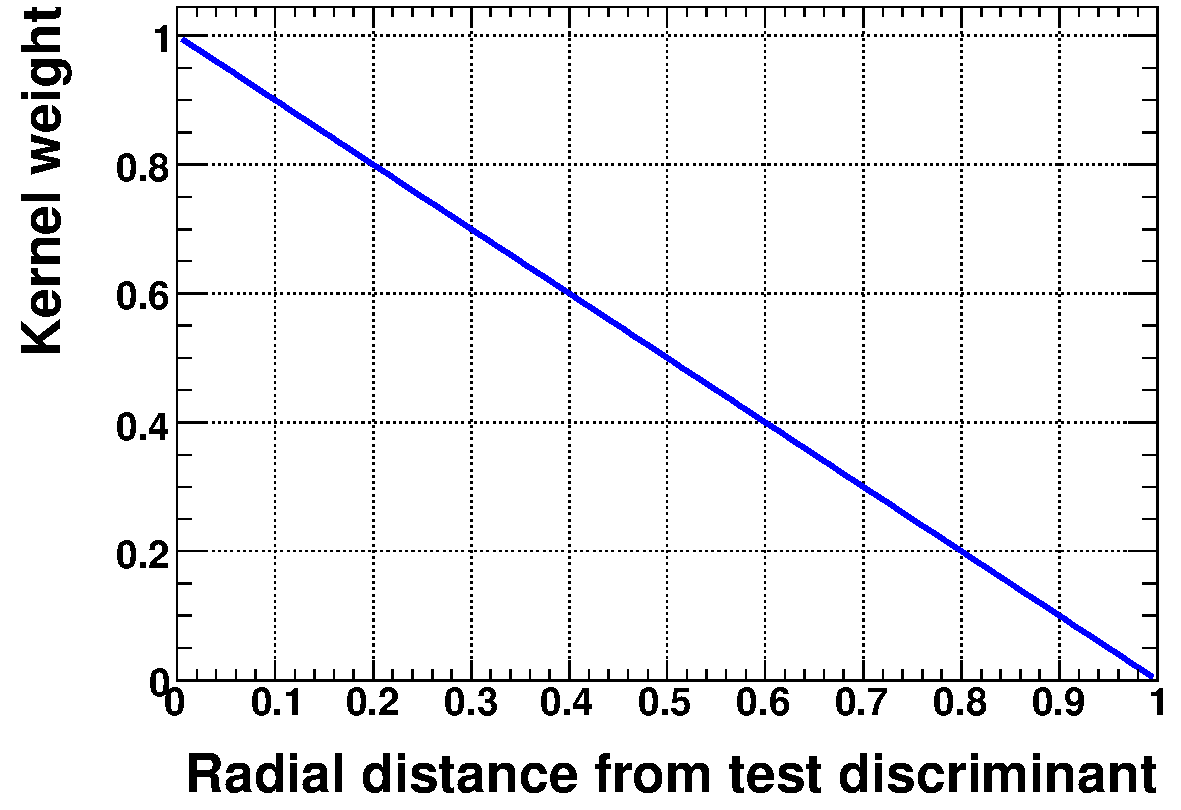
\includegraphics[width=0.49\textwidth]{plots/pders_teepee}
\end{center}
\vspace{-0.5cm}
\caption[.]{Kernel functions (left: Gaussian, right: Teepee) 
 		   used to weight the events that are found 
	      inside the reference volume of a test event.}
\label{fig:pdersKernels}
\end{figure}

\subsubsection*{Regression}

Regression with PDE-RS proceeds  similar to classification. The difference 
lies in the replacement of Eq.~(\ref{eq:PDERSratio}) by the average target value 
of all events belonging to the volume $V$ defined by event $i$ (the {\em test} event)
\beq
\label{eq:PDERSregratio}
	\RPDERS(i,V) = \langle t(i,V)\rangle = 
                   \frac{\sum_{j \in V}{w_{j} t_{j} f(\operatorname{dis}(i,j))}} 
                       {\sum_{j \in V}{w_{j} f(\operatorname{dis}(i,j))}}\,,
\eeq
where the sum is over all training events in $V$, $w_j$ and $t_j$ are the weight and 
target value of event $j$ in $V$, $\operatorname{dis}(i,j)$ is a measure of the distance
between events $i$ and $j$, and $f(\dots)$ is a kernel function.

\subsubsection{Variable ranking}

The present implementation of PDE-RS does not provide a ranking of 
the input variables.

\subsubsection{Performance}

As opposed to many of the more sophisticated data-mining approaches, which 
tend to present the user with a ''black box'', PDE-RS is simple enough that 
the algorithm can be easily traced and tuned by hand. PDE-RS can yield competitive 
performance if the number of input variables is not too large and the statistics
of the training sample is ample. In particular, it naturally deals with complex
nonlinear variable correlations, the reproduction of which may, for example, require
involved neural network architectures.

PDE-RS is a slowly responding classifier. Only the training, \ie, the fabrication 
of the binary tree is fast, which is usually not the critical part. 
The necessity to store the entire binary tree in memory to avoid accessing
virtual memory limits the number of training events that can effectively be 
used to model the multidimensional PDF. This is not the case for the other 
classifiers implemented in TMVA (with some exception for Boosted Decision Trees).

